\subsection{Curved Cantilever Beam Under Point Force}\label{sec:bathe}
%
The curved cantilever in Figure~\ref{fig:bathe} was first studied
by \cite{bathe1979large}, and has become a staple in the literature
on geometrically nonlinear rods. 
This example is selected to demonstrate the path-independence of the \texttt{Init} interpolation.
The undeformed centerline of the cantilever follows a \(45^\circ\) arc with radius \(R\) given by:
\[
\bm{x}_0(\reflenx) = R \sin \reflenx \frac{\pi}{4L}\, \mathbf{E}_1 
                      + R \left(1 - \cos \reflenx \frac{\pi}{4L}\right)\, \mathbf{E}_3.
\]
A point load \(\bm{F} = 600 \, \mathbf{E}_2\) is applied
at the tip, i.e.\ at \(\reflenx = R\).
There is no closed-form solution to the problem, and it is customary
to present the final displacements at the tip:
\[
\Delta x_i \triangleq \mathbf{E}_i \cdot \left(\bm{x}(L) - \bm{x}_0(L)\right).
\]
%
The following parameters are used for the simulations:
\[
\begin{array}{lr}
% Hockling
    R  =& 100 \\ %   ,& A  &= 10 \\
    E  =& 1000 \\ %   ,& I  &= 0.0833 \\
    G  =& 500 \\ %   ,& J  &= 2.16 \\
\end{array}
\qquad\qquad
\begin{array}{ll}
% Hockling
    A  =& 10^4    \\
    I  =& 10^4/12 \\
    J  =& 10^4/6  \\
\end{array}
\]
The analysis uses a discretization with 8 2-node elements.
The analysis is performed twice for each formulation under consideration,
first with 8 equal load increments and then with 10.
The results are presented in Table~\ref{tab:bathe}.
Only the formulations with the \texttt{Init} interpolation
produce the same tip displacement in both load cases, indicating
an artificial path dependence for all other variants.
% 

\begin{figure}
    \centering
    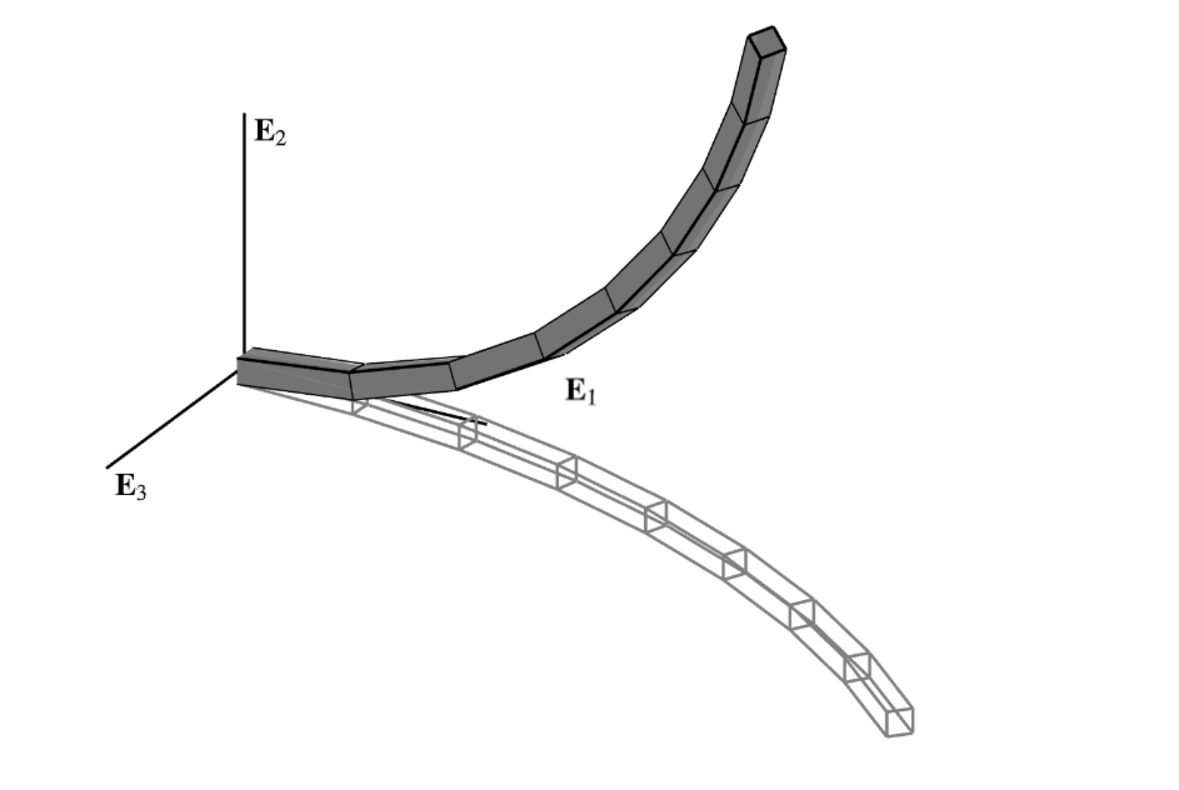
\includegraphics[width=0.6\textwidth]{Examples/frame-1001/Figures/Figure_3}
    \caption{Deformed shape of curved cantilever by \cite{bathe1979large}.}
    \label{fig:bathe}
\end{figure}
%

\begin{center}
\begin{table*}[!h]%
\caption{End displacements \(\Delta \boldsymbol{x}(L)\) of the curved cantilever by \cite{bathe1979large} for a discretization with 8, 2-node elements.}
\label{tab:bathe}
\begin{tabular*}{\textwidth}{@{\extracolsep\fill}cccccccccc@{}}
\toprule
\textbf{Interpolation} & \textbf{Isometry} & \textbf{Parameters} &
\textbf{Steps} & \textbf{Avg. Iter.} & \textbf{Max. Iter.} &
  \(\Delta x_1\) & \(\Delta x_2\) & \(\Delta x_3\)
\\ % 
% tol=1e-16, 8 elements, 2 nodes each
\midrule
  \texttt{None} & \texttt{None} & \texttt{None} &  \hphantom{.}8 & 6.38 & 8 &  -23.477869   &   53.36939  &   -13.487488 \\ 
  \texttt{None} & \texttt{None} & \texttt{None} &             10 & 5.80 & 7 &  -23.477858   &   53.36939  &   -13.487474 \\ 
% \hline
  \texttt{None} & \texttt{SFIN} & \texttt{None} &  \hphantom{.}8 & 6.38 & 8 &  -23.477878   &   53.369398 &   -13.487481 \\ 
  \texttt{None} & \texttt{SFIN} & \texttt{None} &             10 & 5.80 & 7 &  -23.477864   &   53.369395 &   -13.487469 \\ 
  \hline
% \texttt{None} & \texttt{SFIN} & \texttt{Init} &  \hphantom{.}8 & 6.38 & 8 &  -23.477883   &   53.369414 &    -13.487489 \\
% \texttt{None} & \texttt{SFIN} & \texttt{Init} &             10 & 5.70 & 7 &  -23.477862   &   53.369394 &    -13.487472 \\
% \hline
  \texttt{Incr} & \texttt{None} & \texttt{Incr} &  \hphantom{.}8 & 8.38 & 9 &  -23.476519   &   53.369477 &   -13.489989 \\ 
  \texttt{Incr} & \texttt{None} & \texttt{Incr} &             10 & 7.60 & 8 &  -23.476811   &   53.369459 &   -13.489425 \\ 
% \hline
  \texttt{Incr} & \texttt{SFIN} & \texttt{Incr} &  \hphantom{.}8 & 6.38 & 8 &  -23.476522   &   53.369491 &   -13.490001 \\ 
  \texttt{Incr} & \texttt{SFIN} & \texttt{Incr} &             10 & 5.70 & 7 &  -23.476813   &   53.369467 &   -13.489432 \\
  \hline
  \texttt{Init} & \texttt{None} & \texttt{Init} &  \hphantom{.}8 & 8.12 & 9 &  -23.450085   &   53.373025 &   -13.546693 \\ 
  \texttt{Init} & \texttt{None} & \texttt{Init} &             10 & 7.50 & 8 &  -23.450085   &   53.373025 &   -13.546693 \\
% \hline
  %
  \texttt{Init} & \texttt{SFIN} & \texttt{Init} &  \hphantom{.}8 & 6.38 & 8 &  -23.450656   &   53.374198 &    -13.546972 \\
  \texttt{Init} & \texttt{SFIN} & \texttt{Init} &             10 & 5.70 & 7 &  -23.450656   &   53.374198 &    -13.546972 \\
% \hline
  \texttt{Init} & \texttt{SFIN} & \texttt{None} &  \hphantom{.}8 & 6.38 & 8 &  -23.450656   &   53.374198 &    -13.546972 \\
  \texttt{Init} & \texttt{SFIN} & \texttt{None} &             10 & 5.80 & 7 &  -23.450656   &   53.374198 &    -13.546972 \\
\bottomrule
\end{tabular*}
\end{table*}
\end{center}



% \begin{center}
%\begin{table*}[!h]%
%\caption{}
%\label{tab:bathe}
% \begin{tabular}{llll}
% \midrule
% \cite{bathe1979large}                  & -23.5   & 53.4   & 13.4   \\
% \cite{simo1986threedimensional}        & -23.48  & 53.37  & 13.5   \\
% \cite{cardona1988beam}                 & -23.67  & 53.50  & 13.73  \\
% \cite{crisfield1990consistenta}        & -23.87  & 53.71  & 13.63  \\
% \cite{ibrahimbegović1995finite}        & -23.746 & 53.407 & 13.601 \\
% \cite{ibrahimbegović1995computational} & -23.697 & 53.498 & 13.668 \\
% \cite{schulz2001nonlinear}             &         & 53.56  &        \\ % 4-node element
% \cite{makinen2007total}                & -23.696 & 53.497 & 13.668 \\
% \bottomrule
% \end{tabular}
%\end{table*}
% \end{center}
